\chapter{Introduction}\label{sec-introduction}

\section{Oceanic eddies}

Oceanic mesoscale eddies refer to swirling bodies of water that could resist stretching and have semi-diameter ranging from 20 km to 100 km \cite{nencioli2010vector,beron2018enduring}. They carry high concentrations of carbon, chlorophyll, and nutrient, isolate themselves from the surrounding water and have a life circle of several months. Thus, they play a significant role in marine material transport of heat, mass such as nutritive salts, and momentum and have a great impact on global ocean circulation and long-range climate change \cite{mcgillicuddy2007eddy,he2022lagrangian,peacock2013lagrangian,wang2015coherent}. A comprehensive and systematic investigation of vortex characteristics (including statistical characteristics and three-dimensional structures, etc) contributes to the understanding of the oceanic dynamical process.

\begin{figure}[ht]
	
  \centering
  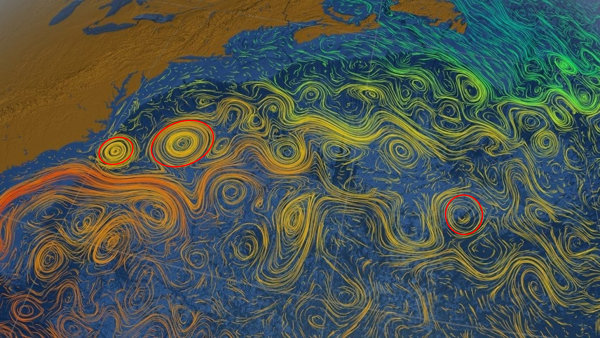
\includegraphics[width=14cm]{chapter/figure/visible eddies and currents in the North Atlantic.png}
  \caption
  {Image of visible eddies and currents photographed by NASA} 
  \label{visible eddies and flow}
\end{figure}


Figure \ref{visible eddies and flow} is a snapshot of Perpetual Ocean which shows ocean surface currents produced by model output (ECCO2). We could observe a lot of spiral-shaped eddies (markded in red circles) which trap certain amount of water inside in the figure.

	
Figure \ref{Plankton Bloom} shows how eddies deflect the density interfaces, deepen or shallow pycnocline (two density surfaces are seasonal thermocline $\rho_1$ and main thermocline $\rho_2$), and generate associated upwelling or downwelling. Thus nutrients can be brought up to the surface and down to the interior during the evolution of the eddies, which means that eddies directly affect the biogeochemistry process.

\begin{figure}[ht]
  \centering
  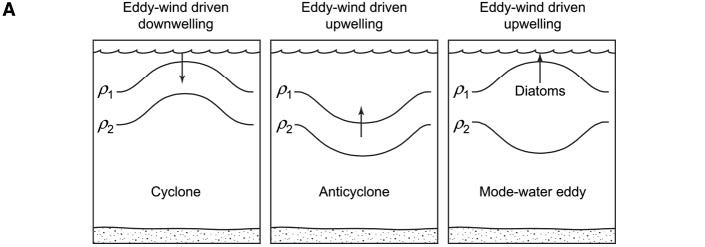
\includegraphics[width=15cm]{chapter/figure/Plankton Blooms.jpg}
  \caption
  {Isopycnal displacements associated with three types of eddies \cite{mcgillicuddy2007eddy}} 
  \label{Plankton Bloom}
\end{figure}

Previous studies have shown that eddy-induced fluid volume zonal transport can reach up to $ 30\sim40 $ Sv, which is as much as the large-scale wind-driven or  thermohaline circulation \cite{zhang2014oceanic}. In figure \ref{zonal transport of fluid carried by mesoscale eddies}, part A of the figure shows us the result of eddy-induced zonal transport per latitude based on the mean eddy propagation speed and trapped fluid volume while part B of the figure illustrates the total meridionally integrated zonal transport induced by eddies (blue curve here represents the westward transport and the red curve represents the eastward transport).The studies serve as the evidence of mesoscale eddies' role in the heat, energy, and flux transport.

\begin{figure}[ht]
  \centering
  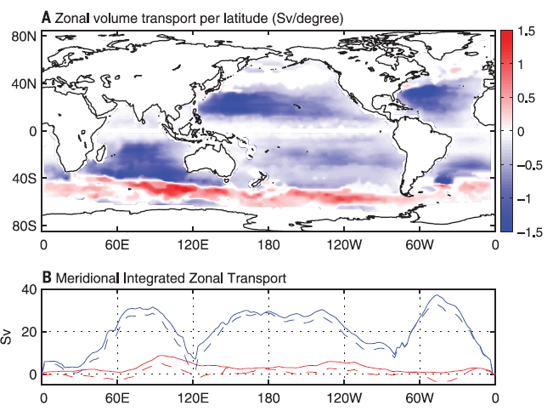
\includegraphics[width=15cm]{chapter/figure/Global distribution of the zonal and meridional transport of fluid trapped by mesoscale eddies.png}
  \caption
  {Global distribution of the zonal water transport carried by eddies 
  \cite{zhang2014oceanic} }
  \label{zonal transport of fluid carried by mesoscale eddies}
\end{figure}

The tremendous advances in ocean observational methods, especially measurements of ocean surface sea level anomaly, and altimetry-derived velocity fields enable the long-term detection of mesoscale vortices. An increasingly high-resolution and submesoscale-permitting ocean circulation model provides a panoramic view of the three-dimensional ocean flow.

Thus, detection and tracking of coherent ocean eddies have increasingly become a research hot spot.  

\section{The flow pattern of the Argentine Basin}\label{flow pattern of the Argentine Basin}

The Argentine Basin region, characterized by its basin structure, exhibits several different types of surface and subsurface currents and unique temperature and salt structures.

The Brazil‐Malvinas region is characterized by the confluence of southward transport Brazil Current (BC) and northward transport Malvinas Current (MC). Previous studies shows that BC transports about 25 Sv ( $ 1 \mathrm{Sv} = 10^6 m^3 s^{-1}$) warm ($\theta > 10^{\circ} \mathrm{C}$) and salt ($S > 35$) water and MC transports about 30-40 Sv cold ($\theta < 7^{\circ} \mathrm{C}$) and fresh ($S < 34.3$) water into the  Brazil‐Malvinas region \cite{jullion2010circulation}. The mixture of these two distinct water bodies would 
generate strong salinity and thermal gradient and cause mesoscale instabilities, which is expected to result in large amounts of oceanic eddies \cite{de2006multi}.

The great variability of the dynamic topography also gives rise to the anisotropic feature in the study region. For example, in the center of the Argentine Basin, Zapiola Anticyclone (ZA) is trapped by a seamount called the Zapiola Rise and the flow greatly inhibits the lateral transport of water, traps water inside, and increases vertical movement such as downwelling transport into the bottom Ekman layer \cite{weijer2020zapiola,frajka2019atlantic,dewar1998topography}.

What is more, the Argentine Basin is regarded as the main channel connecting the Southern Ocean and the Atlantic Ocean, and the properties of water masses inside the Argentine Basin are quite complicated. For example, looking down from the surface, the salinity of the surface-layer water is quite low, and the salinity becomes higher when it mixes with the North Atlantic Deep Water at about 1500-3500 m depth and it becomes a little fresher when it goes down into Antarctic Bottom Water \cite{talley2011descriptive}. The vertical distribution of water bodies is listed in the table \ref{Water mass vertical distribution} \cite{fontela2021anthropogenic}:

\doublerulesep 0.1pt
\begin{table}[htb]
  \centering
 \linespread{1.7}{ {\footnotesize
  \caption{Water mass vertical distribution}\label{Water mass vertical distribution}
\vspace{2em}
  \begin{tabular}{ccc}
  \hline
\noalign{\smallskip}
  \textbf{Water mass} & \textbf{Depth} & \textbf{Density $ \left(\mathrm{kg} \cdot \mathrm{m}^{-3}\right) $} \\
\noalign{\smallskip}
  \hline
  South Atlantic Central Water & 100 - 300 m & $\sigma \le 26.5 $ \\
  Sub Antarctic Mode Water & 300 - 600 m & $ 26.5<\sigma <27.1 $  \\
  Antarctic Intermediate Water & 600 - 1000m & $ 27.1<\sigma <27.4$ \\
  North Atlantic Deep Water & 1000 - 400 m & $ 27.4<\sigma < 45.90$ \\
  Antarctic Bottom Water & towards the sea floor & $ \sigma \ge 45.90$ \\
  \hline
\noalign{\smallskip}
  \end{tabular}
  }}
\end{table}

Due to the dynamic changes of the current and strong mixing in the study region, lots of energetic mesoscale eddies having great impact on heat and salt budgets were observed.


\section{Traditional vortex detection methods}\label{Eulerian representation}\label{Eulerian methods}

Traditional automated Eulerian eddy detection methods can be divided into three types \cite{nencioli2010vector}: physical parameter-based algorithm using the value exceeding a threshold to identify eddies, flow geometry-based methods focusing on the morphology of the instantaneous streamlines to extract vortices, and hybrid approach taking both the physical parameters and geometric features into consideration. 

McWilliams developed the earliest automatic eddy detection algorithm for decaying two-dimensional turbulence. The detection procedure is as follows: at first, we pick a two-dimensional extreme (maximum or minimum) in vorticity ($\xi$) as their center, and then identify the boundary as the points set with the criterion of $\frac{\xi}{\xi_c} \geqslant \Delta$ (${\xi_c}$ is the vorticity of the vortex center and $\Delta$ is the limiting value and 0.2 might be a satisfactory value) as shown in figure \ref{Closed vorticity contour in the turbulence flow}. Besides setting vorticity as the physical parameter, geometric characteristics are also taken into consideration: several shape quantities are raised to ensure that the boundary and interior of the candidate eddy should not depart excessively from asymmetry \cite{mcwilliams1990vortices}. This method belongs to the hybrid one.

\begin{figure}[ht]
  \centering
  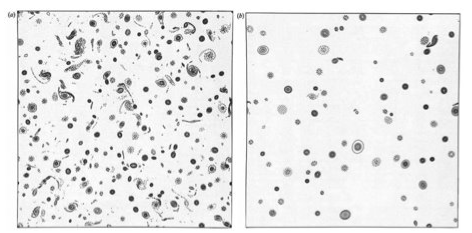
\includegraphics[width=15cm]{chapter/figure/closed vorticity contour in the turbulence flow.png}
  \caption
  {Closed vorticity contour in the turbulence flow 
  \cite{mcwilliams1990vortices} }
  \label{Closed vorticity contour in the turbulence flow}
\end{figure}

Among the overall methods, the most popular Eulerian methods are the SSHA method(\cite{roemmich2001eddy}), and Okubo-Weiss method. SSHA method considers sea level anomalies exceeding a threshold as an eddy and consider the local minimum (maximum) of SSH for cyclonic (anticyclonic) eddies \cite{chelton2011global}. However, this method lacks the ability to distinguish wave-like structures with eddies. Okubo-Weiss method detects eddies based on Okubo-Weiss parameter, W, which defines eddies by stretch ($s_{s}$), shear ($s_{n}$), and relative vorticity ($\omega$) in the flow field and the rotation-dominated case ($W < 0$) is considered as vortex \cite{calil2008eddy,chelton2007global}. $W=-2 \times 10^{-12} \mathrm{~s}^{-2}$ contours is used to extract eddies in global study.

\begin{equation}
    W=s_{s}^{2}+s_{n}^{2}-\omega^{2} 
\end{equation}

\begin{equation}
    s_{n}=\frac{\partial u^{\prime}}{\partial x}-\frac{\partial v^{\prime}}{\partial y}, \quad s_{s}=\frac{\partial v^{\prime}}{\partial x}+\frac{\partial u^{\prime}}{\partial y}, \quad w=\frac{\partial v^{\prime}}{\partial x}-\frac{\partial u^{\prime}}{\partial y}
\end{equation}

Via geostrophic balance, $u^{\prime}$ and $v^{\prime}$ may be calculated by the gradient of sea level anomaly.

\begin{equation}
    u^{\prime}=-\frac{g}{f} \frac{\partial(SLA)}{\partial y}, \quad v^{\prime}=\frac{g}{f} \frac{\partial(SLA)}{\partial x}
    \label{Geostrophic anomaly velocity}
\end{equation}

\begin{figure}[ht]
	\centering
	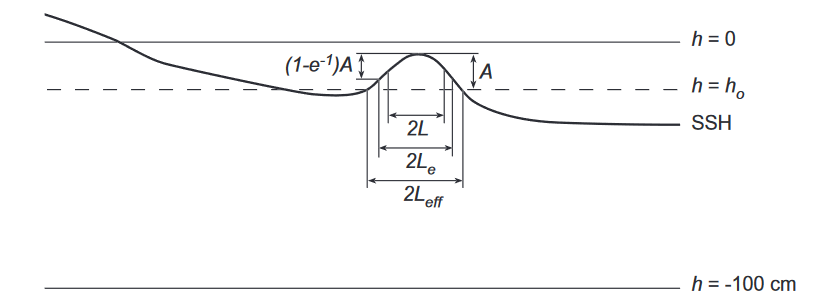
\includegraphics[width=15cm]{chapter/figure/A schematic summary of the automated eddy identification procedure for the case of an anticyclonic eddy.png}
	\caption
	{A schematic summary of the automated eddy identification procedure for the case of an anticyclonic eddy 
		\cite{chelton2011global} }
	\label{A schematic SSHA anticyclonic eddy}
\end{figure}

However, above Eulerian diagnostics are unreliable since they are not objective and depend on thresholds. Being not objective means that the results would perform differently when viewed from different reference frames. In other words, the existence of the eddy is questionable and the transport of material carried by eddy is not guaranteed to be coherent. Depending on thresholds signifies that the results of the detection would vary a lot and the boundary would disagree with each other when choosing different thresholds. In the following chapter \ref{Coherent vortices and geodesic theory}, we would turn to a new concept of Lagrangian coherent structures and how it is related to the detection of oceanic eddies.

\clearpage 

\section{Lagrangian coherent structures}\label{Coherent vortices and geodesic theory}

Recently, breakthroughs at the crossroads of nonlinear dynamical systems theory and fluid dynamics has promoted the application of detecting the vortices in a variety of fields. As shown in figure \ref{Lagrangian coherent structures}, in the field of dynamical systems, Lagrangian coherent structures (LCSs) refer to material lines or surfaces that attract, repel, or shear the most, which uncover the geometric property of the flow field (repelling LCSs tends to induce local stretching, thinning, and folding happen along attracting LCSs boundary, and shear LCSs describe swirling pattern \cite{haller2000lagrangian}), and thus play a significant role in the study of chaotic advection and material mixing \cite{haller2015lagrangian,aref2017frontiers,bettencourt2012oceanic}. Material coherence is observable everywhere in nature: Great Red Spot  photographed by Voyager 1 in 1979 and processed by Bjorn Jonsson as shown in figure \ref{red spot}. Because LCSs could influence the particles around them more than others, which means that this structure is not transient, thus a structure is considered coherent if it lasts a long time in the flow of the observed fluid \cite{peacock2013lagrangian}. In other words, LCSs could not be crossed by material and act as transport barrier, thus providing solid framework to detect coherent eddies.      

\begin{figure}[ht]
  \centering
  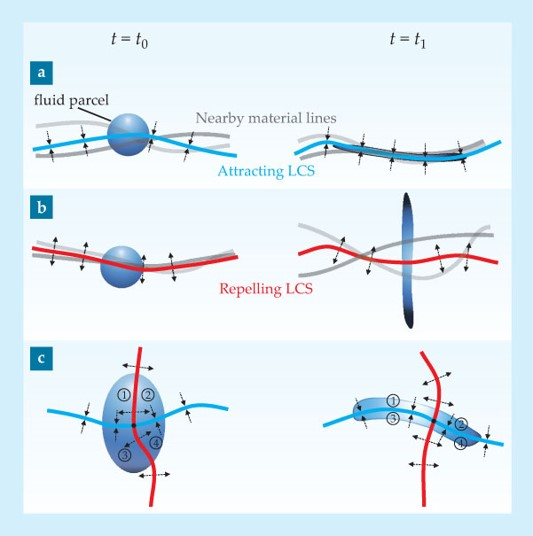
\includegraphics[width=7cm]{chapter/figure/Lagrangian coherent structures.jpg}
  \caption
  {Lagrangian coherent structures
  \cite{peacock2013lagrangian}} 
  \label{Lagrangian coherent structures}
\end{figure}

\begin{figure}[ht]
  \centering
  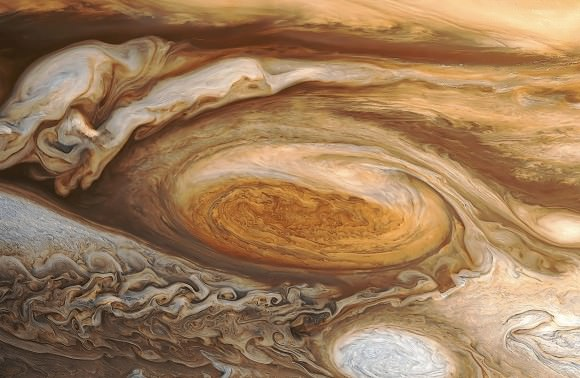
\includegraphics[width=13cm]{chapter/figure/coherent structure and red spot.jpg}
  \caption
  {Observable Coherent Lagrangian patterns(The Great Red Spot)
  \cite{haller2015lagrangian}} 
  \label{red spot}
\end{figure}

Instead of observing fluid properties from a fixed frame in chapter \ref{Eulerian representation} (Eulerian representation), Lagrangian dynamics focus on the motion of specific parcels of fluid and follow them through space \cite{price2006lagrangian}. Assessment of flow patterns from a single tracer is impractical because of the sensitivity of fluid-particle trajectories to initial conditions; however, LCSs provide a solid framework of material surfaces and thus enable the comparison of models and other observational data\cite{haller2015lagrangian}. 

However, LCSs in ocean turbulence are not well-defined and interpreted as material loops showing little deformation, no filamentation, and consistent area during the so-called LCSs life cycle, which would last for several weeks to several months. LCSs are believed to be bounded by uniformly stretching fluid line and maintain the arc length during the transport period. Such coherent structures will confine mixing and material exchange between the water body trapped inside and ambient ocean turbulent flow and thus quantify important aspects of material transport\cite{haller2015lagrangian}.

Recently, several Lagrangian methods have been developed to accurately predict the material transport barrier in geophysical flows: ridges of finite-time
Lyapunov exponent (FTLE) \cite{shadden2005definition, haller2011lagrangian}, and finite-size Lyapunov exponent (FSLE) \cite{aurell1997predictability, joseph2002relation, d2004mixing}. Haller proposed that the ridge of FTLE would be an indicator of hyperbolic LCSs (repelling in forward time and attracting in backward time) \cite{haller2001distinguished}. However, it still remains uncertain about the relationship between FTLE or FSLE with LCS and some counterexamples have doubted the robustness of the detection method \cite{haller2011variational, karrasch2013finite}. As shown in figure \ref{LCS and FTLE}, there is an observable repelling LCS along y-axis in the nonlinear strain flow while FTLE ridges are not detected in this case (constant forward FTLE field) \cite{haller2011variational}. In classic dynamical systems, this recurrent structure is called the saddle fixed point.

\begin{figure}[ht]
  \centering
  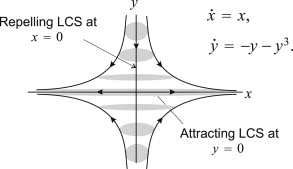
\includegraphics[width=12cm]{chapter/figure/mismatch.jpg}
  \caption
  {A mismatch between a repelling LCS and FTLE ridges\cite{haller2011variational}
  \label{LCS and FTLE}
  }
\end{figure}

In order to reduce the false positive and false negative results in coherent structure detection, a redefinition with rigorous mathematics is needed. 

\clearpage

\section{Dynamic Mechanisms of the  Mesoscale Eddy}

According to previous studies, the properties and formation of eddies were strongly related to the evolution of baroclinic instability caused by vertical velocity shear between different layers \cite{feng2021four,verma2021lagrangian}.

%and the existing distinct seasonal variation in eddy kinetic energy (EKE) may be related to the seasonal circle of vertical velocity shear change.

Complex flow-vortex interactions with strong currents near the western boundary could also explain the complicated LCSs in the study region.
 
Other dynamical factors such as mixed layer instabilities, frontal dynamics, buoyancy anomalies produced by sea ice leads and so on could also affect the formation and evolution process of LCSs \cite{mukiibi2016three,cohanim2021dynamics}.

How relative wind stress acts on eddies is controversial: some researchers think that it would depress the development of eddies and performs as the ``killer" of eddies' kinetic energy \cite{xu2016work,renault2019remarkable}; however, an updated study have demonstrated that eddies can response and adjust to the wind and the work done by relative wind stress on eddies could turn from negative to positive after the "inflection point" \cite{teng2021does}.

\clearpage

\section{Main content and Organization of the paper}

As mentioned above, studies of mesoscale eddies are now the research hotspots due to the importance of eddies' role. However, studies of basic statistical characteristics of the vortex, the three-dimensional structure of the vortex, and its influence on the vertical distribution of temperature and salt are not very clear in Argentine Basin. We want to understand the following questions: (1) How deep do the ocean eddies extend? (2) What is the shape of ocean eddies? (3) How many eddies could be detected and what are the characteristic features of the ocean eddies? (4) Given the same domain and same velocity field generated by the numerical model, how different it will be when different methods are adopted?

The thesis includes six chapters, and it starts with a brief introduction to the ocean eddies detection methods and flows pattern of the Argentine Basin. Chapter Two mainly discuss the detailed setup process of the eddy’s detection.

Chapters Three to Five contain the main body of this thesis and cover the eddies properties, three-dimensional eddies profile, and comparison of several different methods in the eddy detection process. The last chapter draws a general conclusion from the above content and outlines several future research directions.

To be specific, Chapter Two gives mathematical images and formulas of nonlinear dynamics and geodesic theory and its application to geostrophic flow. Since the content is not intuitive enough, someone who is not familiar with the notion may skip this chapter and backtrack the chapter as a reference when needed. What is more, we also discuss the drawback of traditional Eulerian method, which is the base of Chapter Three.

Chapter Three focuses on the comparison of Eulerian methods and Lagrangian methods and verifies the robustness of LAVD method. The similarities and differences between these results are discussed here.

Chapter Four concerns the statistical quantity of the ocean eddies such as their radius, polarity and population. We show that most eddies maintain their coherent feature during the transport, which lays a solid foundation for accurately quantifying the eddies-induced transport in Argentine Basin.

In Chapter Five, we explore the three-dimensional structure of the vortex and discuss the vertical extension of eddies from the surface to subsurface. 

Chapter Six makes a conclusion of the work and provides an outlook and forecast of possible future work.

\newpage
